Der er en række interessenter at tage hensyn til, når det kommer til, hvordan et folkeskoleskema skal planlægges. For at lave et velfungerende skemalægningsprogram til folkeskoler, skal der tages højde for de forskellige interessenter, der bliver påvirket af programmets produkt. I følgende afsnit vil forskellige interessenters påvirkning af en softwareløsning undersøges samt deres indflydelse. 


Kommunernes mål er at forbedre elevernes læring, samt overholde undervisningsministeriets krav. Både uddannelsesministeriet og kommunen stiller krav til hvilke fag, som skemaet består af, samt antallet af undervisningstimer, der skal afsættes til de forskellige fag. Kommunernes påvirkning af en softwareløsning ville være minimal, så længe deres opstillede krav overholdes af programmet.\footfullcite{lov2016}


Skolelederen arbejder ud fra et budget, som er tildelt af kommunen, og er derfor interesseret i at optimere mængden af ydelser, dette budget finansierer. En softwareløsning der reducerede timeantallet brugt på skemalægningsprocessen kunne have en stor interesse hos skolelederen, da dette vil tillade budgettet at bruge penge andre steder på skolen, hvor det vil gavne mere. Skolelederen har stor indflydelse på om programmet bliver implementeret, da det er skolelederens beslutning om det er gavnligt at investere i programmet. Det ville også kræve at programmet ikke kræver flere mandetimer end manuel skemalægning, eller producerer en løsning, som ikke er holdbar. Skolelederen har ingen interesse i at investere i en softwareløsning, som skaber flere problemer end den løser. En softwareløsning som producerer et velfungerende skema er for skolelederen vigtigt, da det er skolelederen, der står til ansvar, hvis programmet viser sig at være en dårlig investering.\footfullcite{interview}


Lærerne bruger tid og kræfter på skemalægningsprocessen.\footfullcite{interview} En softwareløsning vil lette arbejdsbyrden fra lærernes skuldre og ville tillade, at de kan fokusere fuldt ud på undervisningen. Lærerne vil have stor indflydelse på, hvordan en softwareløsning ville komme til at se ud, da det er dem som lægger skemaet. Deres indflydelse påvirker om en softwareløsning vil blive implementeret på en skole, da softwareløsningen skal kunne opfylde lærernes betingelse for et skoleskema fejlfrit. Da lærerne ikke er interesseret i et program, som skaber flere problemer for dem, end det reelt løser. Lærernes betingelser til en softwareløsning består i at få et optimeret skemaet, så eleverne er fokuseret i undervisningen, og at underviserens forberedelsestimer er samlet. Derudover har Sofiendalskolen fundet ud af, at eleverne har besvær med at koncentrere sig i de tungere fag over middag. Dette giver en præference, hvor de tunge fag placeres før middag. En softwareløsning ville også have en stor påvirkning på lærernes hverdag, da de arbejde ud fra skoleskemaet og problemer, som skoleskemaet skaber, vil have direkte påvirkning på lærerne.\footfullcite{interview}


Eleverne har ingen interesse i en softwareløsning og deres indflydelse, på hvordan den endelige løsning kommer til at se ud, er minimal, da de ingen indflydelse har i skemaplanlægning. Eleverne vil dog muligvis blive påvirket af en softwareløsning, skemaet potentielt bliver bedre ved softwareløsningen. Et dårligt planlagt skema vil gøre at de f.eks. ingen energi har til at komme igennem dagen, hvis der bliver lagt tunge fag sidst på dagen.


Forældrenes interesse er baseret ud fra den påvirkning skemaet har for deres børn. Børnenes faglige trivsel i skolen er vigtigt for forældrene, og et optimeret skema vil hjælpe barnet med at få bedst muligt fagligt udbytte af skoledagen. Forældrene har dog ingen påvirkning på, hvordan skemaet bliver lagt og vil derfor ikke opdage, hvis skolen begynder at bruge en softwareløsning til at planlægge deres børns skemaer.\footfullcite{interview}

For at overskueliggøre de forskellige interessenter og deres indflydelse på, hvordan skemaet bliver bygget, og hvilken påvirkning skemaet vil have på dem, kan de forskellige interessenter opstilles i et skema som ses på figur~\ref{fig:interessenter}.
\begin{figure}[!h]
  \centering
  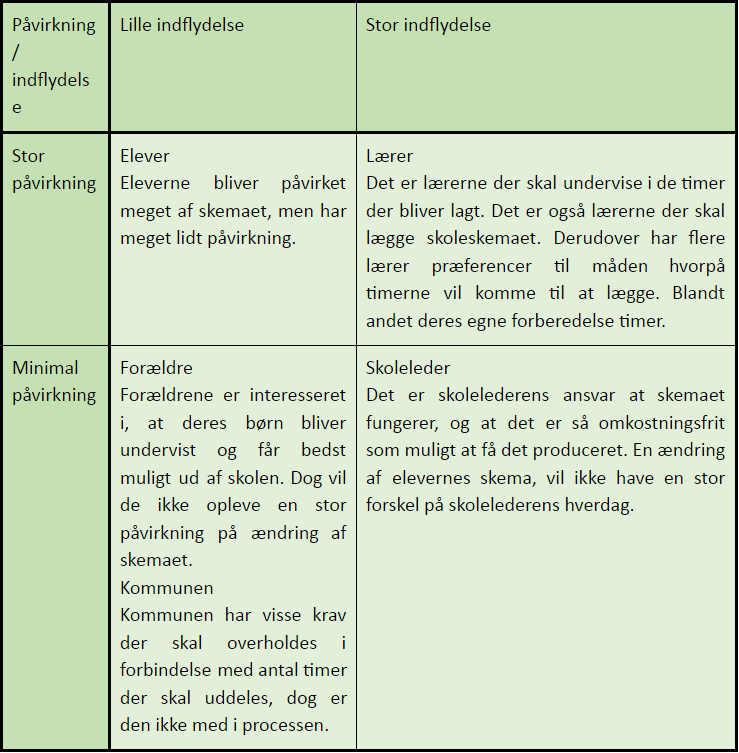
\includegraphics[width=\textwidth]{partials/graphics/interessentanalyse.png}
  \caption{Model over de indblandede interessenter.}
  \label{fig:interessenter}
\end{figure}
